% !TeX encoding=utf8
% !TeX spellcheck = en-US

\chapter{Classes}

All classes are organized in 3 folders: domain, view and custom. Domain contains all classes that purely contain some algorithm logic. View contains classes that are responsible for the GUI and custom also contains GUI classes, but only menu items and tabs which are created by the Factory. Each folder has its own namespace.

\begin{figure}[h]
	\centering
	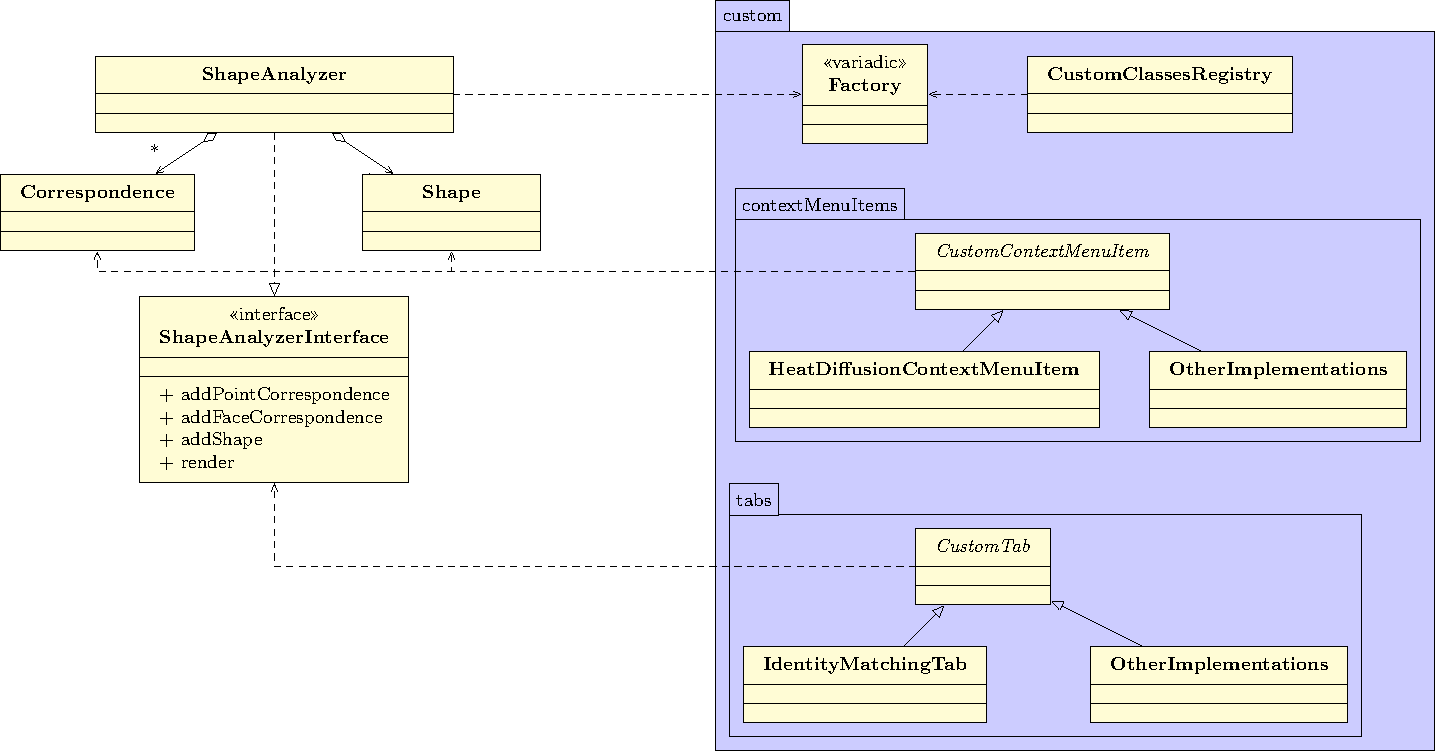
\includegraphics[width=\textwidth]{images/diagram.pdf}
	\caption{UML diagram of the most important classes in view and custom.}
\end{figure}

\section{ShapeAnalyzer}
\label{sec:ShapeAnalyzer}

The ShapeAnalyzer is the main application and manages all user input as well as the existing Shapes and Correspondences. The ShapeAnalyzer should only be changed if really necessary. It is also a QWidget, so it can (and should) be used as the parent for further QWidgets or Qt objects that have a parent widget input. All new Shapes and Correspondences have to be added through this main application and not by directly adding them into the data structures (which is not possible most of the time anyway) in order to keep the whole application up-to-date.

\subsection{ShapeAnalyzerInterface}
\label{subsec:ShapeAnalyzerInterface}

The ShapeAnalyzerInterface is an interface that provides functions to add new Shapes, Correspondences and Render the GUI, basically everything that the custom objects are allowed to do. The custom objects only get a reference to the interface. Theoretically the ShapeAnalyzerInterface can be forcefullly cast into a ShapeAnalyzer object but you should think about whether there might be a different solution. It also prevents cyclic dependencies.

\section{Shape}
\label{sec:Shape}

A Shape contains the mesh data as well several VTK related objects. It has a unique id and a (not necessarily unique) name. The data (\href{http://www.vtk.org/doc/nightly/html/classvtkPolyData.html}{vtkPolyData} object) can be obtained through \texttt{getPolyData()}. Additionally to some self-explanatory functions the surface can be colored with \texttt{setColoring}, see \ref{subsec:Coloring}.

\subsection{Coloring}
\label{subsec:Coloring}

Coloring is a struct in the Shape class. It contains a Type and a vtkDataArray. Either Type is possible as Point or Face. Then the vtkDataArray has to have as many entries as the shape has vertices or faces respectively and every vertex or face will be colored with the value(s) in the same row as their id. It is not possible (to my knowledge) to leave some vertices or faces uncolored. The possible Types are:

\begin{itemize}
	\item \texttt{\textbf{Coloring::Type::PointScalar/FaceScalar} vtkDoubleArray} The minimum value will be blue, the maximum red and all values inbetween have a smooth color gradient.
	\item \texttt{\textbf{Coloring::Type::PointRGB/FaceRGB} vtkUnsignedCharArray} Set the number of components of the array to 3 with \texttt{SetNumberOfComponents(3)}, the components will be interpreted the R, G and B parts and have to be values between 0 and 255. 
	\item \texttt{\textbf{Coloring::Type::PointSegmentation/FaceSegmentation} vtkIntArray} Every integer denotes one region that will be colored in the same color. VTK will automatically color in a way that allows to differ separate regions. If the coloring is set to an segmentation, the region can be extracted as a new shape in the GUI.
\end{itemize}

These are just the standard behaviors of each type. The vtkMapper and vtkLookUpTable of every Shape have more options that can be explored. 

\begin{figure}[h]
	\centering
	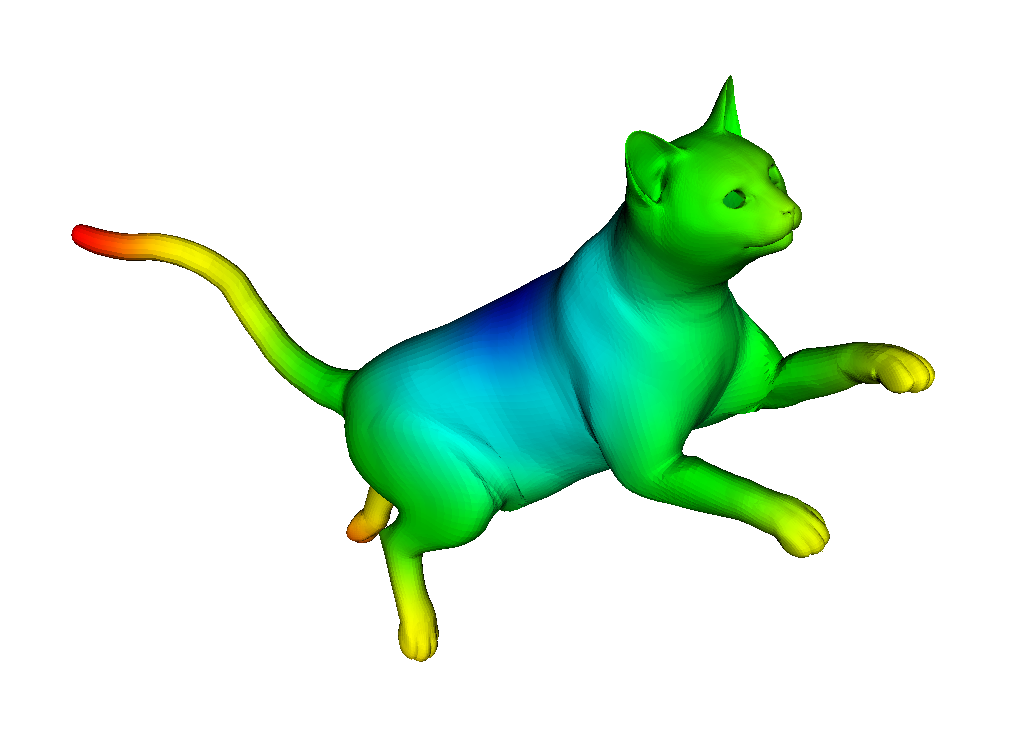
\includegraphics[width=0.3\textwidth]{images/scalar.png}
	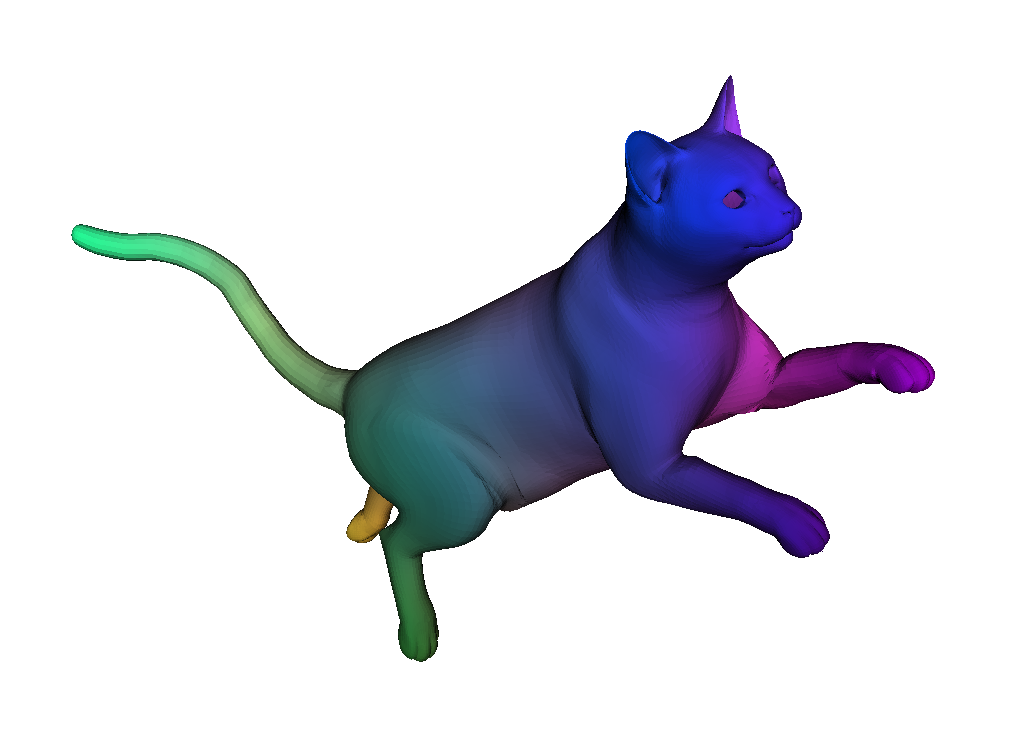
\includegraphics[width=0.3\textwidth]{images/rgb.png}
	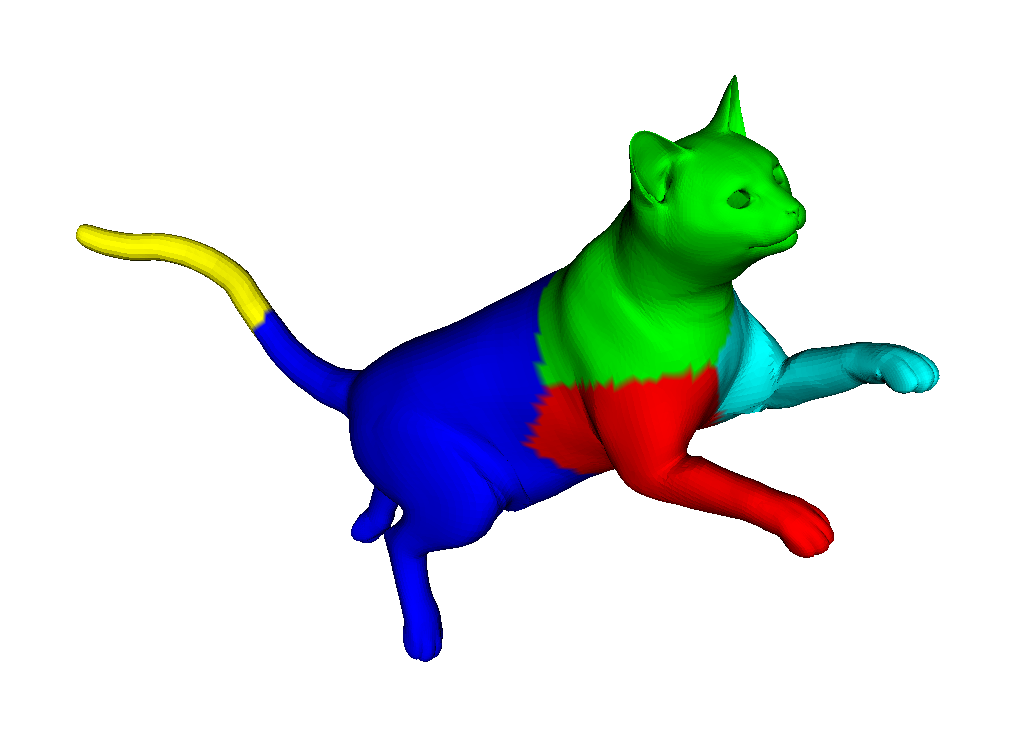
\includegraphics[width=0.3\textwidth]{images/segmentation.png}
	\caption{(i) PointScalar, (ii) PointRGB using the coordinates as RGB values, (iii) PointSegmentation}
\end{figure}

\section{Correspondence}
\label{sec:Correspondence}

A Correspondence is a set of tupels, each containing a shape and an id. There are PointCorrespondences and FaceCorrespondences, the id either belonging to a vertex or a face. The tupels are realized as two vectors where objects in the same row belong to the same tupel. Correspondences can be visualized in the GUI with corresponding VisualCorrespondence objects which are organized (and created) by the ShapeAnalyzer. 

\section{Factory}
\label{sec:Factory}

The Factory is responsible for automatically creating objects of Custom classes (see chapter \ref{chap:Customs}) and making them visible in the GUI. It is a variadic template that allows to specify the number and type of input parameters the constructors of those objects will get. It is realizing the Factory (you might have guessed it from the name) and the Singleton design pattern. 

\begin{mdframed}
If you only want your menu item / tab to appear in the GUI, no deeper knowledge of the Factory is required. Take a look at chapter \ref{sec:RegisterCustoms}. 
\end{mdframed}

\begin{lstlisting}[style=lstStyleCpp, caption={Factory.h}]
template<class T, class... Args>
class Factory {
    ...
    /// \brief Returns the unique instance of Factory<T>.
    /// \details This is the only way to obtain the Factory object for type T.
    static Factory<T, Args...>* getInstance() {
        static Factory<T, Args...> instance;
        return &instance;
    }
    ...
};
\end{lstlisting}

Due to the Singleton pattern there is only one Factory instance of every type. You can retrieve it by calling Factory<T, Args...>::getInstance() with the right template parameters. For example for CustomContextMenuItems there exist this Factory: 

\begin{lstlisting}[style=lstStyleCpp, numbers=none]
typedef Factory<CustomContextMenuItem, shared_ptr<Shape>, ShapeAnalyzerInterface*> CustomContextMenuItemFactory;
\end{lstlisting}

This Factory can produce CustomContextMenuItem objects that get a Shape and a ShapeAnalyzerInterface pointer as input parameters. As CustomContextMenuItem is an abstract class, the concrete classes have to be registered with a string identifier and a label. The string identifier has to be unique among all registered classes, the label will be shown in the GUI. 

\begin{lstlisting}[style=lstStyleCpp, caption=Factory.h]
template<class C>
    void Register(const string& identifier, const string& label) {
        // inserts a pair consisting of the identifier and a c++11 lambda 
        // expression calling the constructor of class C into the map 	
        // constructors
        function<T*(Args...)> constructor([](Args... args)->T* 
        		{ return new C(args...); });
        contructors_.insert(pair<string, function<T*(Args...)
        		>>(identifier, constructor));
        
        labels_.push_back(pair<string, string>(identifier, label));
        labelIndex_.insert(pair<string, int>(identifier, labels_.size() - 1));
}

T* create(const string& identifier, Args... args) {
        // execute create function pointer given the arguments in tuple args.
        return contructors_.at(identifier)(args...);
    }
\end{lstlisting}

The register function is a template taking the concrete class  as the template parameter \texttt{C}. It will create and store a lambda expression that calls the constructor of \texttt{C} with input parameters that were given as template parameters to the Factory template. Afterwards the create function will take the identifier and input parameters and use the stored constructors to create new objects. As the identifiers are stored separately, they can be used to automatically create objects of all registered classes. This happens when the menu is called.

\begin{lstlisting}[style=lstStyleCpp, numbers=none]
CustomContextMenuItemFactory::getInstance()>
Register<VoronoiCellsContextMenuItem<GeodesicMetric>>
("voronoicells_geodesic", "Segmentation>>Voronoi Cells>>Geodesic");
\end{lstlisting}

The label parameter allows to create layered menus. For menu items the label will be separated at every \texttt{>>}, creating a new sub menu. Menu items that have the same label up to some level will be put in the same sub menu. For tabs the label has to start with \texttt{"Shapes>>"} or \texttt{"Correspondences>>"} and no further sub menus will be created. 

\begin{figure}[h]
	\centering
	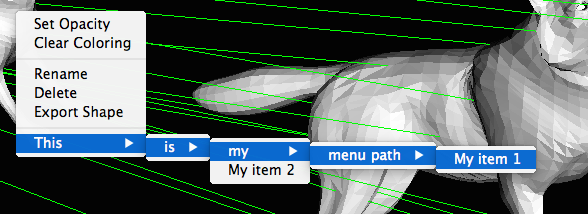
\includegraphics[width=0.8\textwidth]{images/menu.png}
	\caption{The label "\texttt{This>>is>>my>>menu path>>My item 1}" will produce a menu like this.}
\end{figure}

\begin{figure}[h]
	\centering
	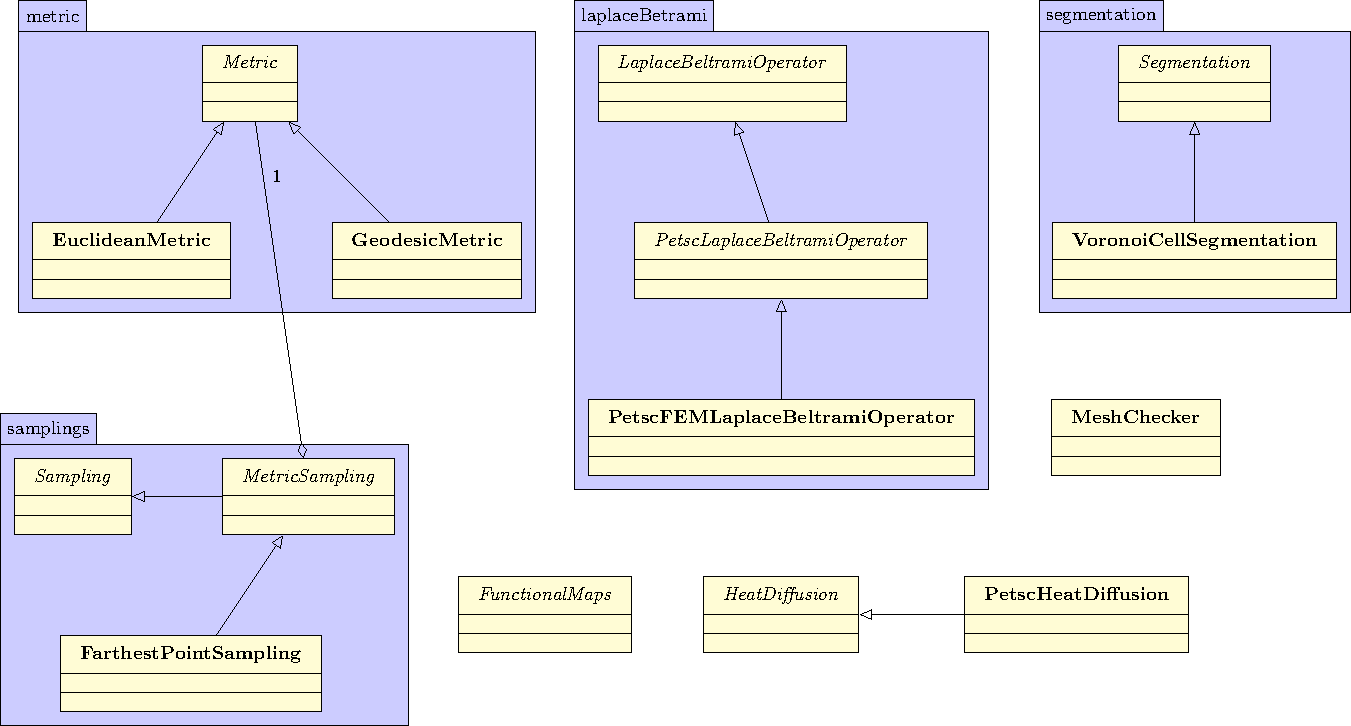
\includegraphics[width=\textwidth]{images/diagram2.pdf}
	\caption{Subset of classes in the domain folder.}
\end{figure}

\section{Domain}

The domain folder consists of several subfolders which contain different kinds of classes that inherit from the same abstract class or belong together somehow. Feel free to add more folders if you think it makes sense. Each folder has its own namespace and Error class (see \ref{sec:Errors}).





